\documentclass{article}
\usepackage{graphicx} % Required for inserting images
\usepackage[top=1in,bottom=1in,left=1.2in,right=1.2in]{geometry}

\title{Homework 5 Template}
\author{Khushi Shelat  \and Justin Zhou}

\date{}

\setcounter{section}{1}

\begin{document}
\maketitle
\thispagestyle{empty}
\pagestyle{empty}

% \section{}
\section{Prompt Engineering}
\subsection{}
Why did the $DONALD\_TRUMP\_PROMPT\_ENGINEERED\_1$ prompt work much better than the $DONALD\_TRUMP\_PROMPT$ prompt?\\ 

The prompt $DONALD\_TRUMP\_PROMPT\_ENGINEERED\_1$ worked better than the initial $DONALD\_TRUMP\_PROMPT$ because it provides a more explicit and focused instruction to the model. $DONALD\_TRUMP\_PROMPT\_ENGINEERED\_1$ starts with a statement that sets the context explicitly: "On the topic of {input}, Donald Trump was quoted as saying." This helps the model understand that it needs to return an actual quote, rather than a guess on what Donald Trump would say. It then says it in first person rather than a different perspective. 

\subsection{}


Report $MOVIE\_SENTIMENT$ prompt and $POSITIVE\_VEBALIZERS$ and\\ $NEGATIVE\_VERBALIZERS$\\
\emph{Response}: \\ 

Our movie sentiment prompt is as follows: "Analyze the following product review and determine if the sentiment is positive or negative: {input}. Return answer in single word as either positive or negative:". We also reordered the code slightly in terms of how we handled $POSITIVE\_VERBALIZERS$ and $NEGATIVE\_VERBALIZERS$ in relation to this prompt. In the final version, we received an accuracy of 126 / 200 with positive verbalizers including "['positive', 'interesting', 'pretty good', 'quite fun', 'highly recommend', 'a classic']" and negative ones including "'['negative', 'propaganda', 'not good']". We found that the model sometimes misinterpreted the prompt and summarized in a full set of sentences the movie review, rather than responding just with 'positive' or 'negative', which is why we added additional keywords. 

\section{Few Shot Prompting}
\setcounter{subsection}{2}
\subsection{}
Come up with 3 more arbitrary tasks, where a zero-shot prompt might not suffice, and a few-shot prompt would be required. Provide a short write up describing what your tasks are. Provide examples of a zero-prompt not working for it. Then, show us your few-shot prompt and some results. Be creative and try to pick 3 tasks that are somewhat distinct from each other!\\
\emph{Response}: 

Our three tasks were (1) identifying the genre of a movie given a movie title, (2) identifying the programming language of an input code snippet, and (3) identifying the author of a given book title. In the first task, we demonstrate that the few-shot prompt is able to specifically return "Romance" on its own for "The Notebook" as an input, whereas the zero-shot prompt assumes the notebook is a novel. For the second task, only the zero-shot prompt correctly responds with 'Python'. For the third task, the zero-shot prompt talks only about Percy Jackson as a character when prompted with "Percy Jackson", but the zero-shot prompt answers correctly with Rick Riordan as the author. Furthermore, we noted that including diverse authors was important because in practice, the ChatGPT model was less likely to correctly guess the author of novels written by immigrants for example, in both the zero and few shot case. 


\section{Prompting Instruction-Tuned Models}
\setcounter{subsection}{1}
\subsection{}
Come up with 3 more arbitrary tasks, where the non-instruction-tuned model might not suffice, and an instruction-tuned model would be required. Provide a short write up describing what your tasks are. Provide examples of a prompt not working on a non-instruction-tuned model. Then, show us your instruction prompt on an instruction-tuned model and some results. Be creative and try to pick 3 tasks that are somewhat distinct from each other!
\\ \emph{Response}:

Our three tasks for prompting instruction-tuned models were (1) coming up with a list of related words given a word, (2) coming up with a related movie title given a subject, and (3) classifying the food group of an input food item. Now, we'll go through each of these tasks and show how the instruction-tuned model performs better than the non-instruction-tuned model. To keep things uniform, we used the same prompt for both models for each task.\\

\textbf{Task 1: Related Words}\\\\
Our prompt for this task was "Give me a list of related words to the following word: \{input\}"\\
\indent Here are the results for the input, 'guitar':\\
\indent \indent Non-instruction-tuned model: 'guitar'\\
\indent \indent Instruction-tuned model: 'guitar, strum, pluck, strumming, chord, melody'\\\\
\indent Here are the results for the input, 'hamburger':\\
\indent \indent Non-instruction-tuned model: 'The word hamburger is a noun.'\\
\indent \indent Instruction-tuned model: 'burger, sandwich, bun, meat, patty, cheese'\\\\
\indent And here are the results for the input, 'wizard':\\
\indent \indent Non-instruction-tuned model: '''\\
\indent \indent Instruction-tuned model: 'magician, sorcerer, witch, warlock, wizard'\\\\
We can see that, in all three cases, the instruction-tuned model performs better than the non-instruction-tuned model. The non-instruction-tuned model does not even return a list of related words for the first and third inputs, and for the second input, it returns a sentence that is not related to the input at all. The instruction-tuned model, on the other hand, returns a list of related words for all three inputs.\\

\textbf{Task 2: Related Movie Titles}\\\\
Our prompt for this task was "You are a bot that generates action movie titles given a subject. Your subject is \{input\}."\\
\indent Here are the results for the input, 'aliens':\\
\indent \indent Non-instruction-tuned model: 'You are a bot that generates action movie titles given a subject. Your subject is aliens.'\\
\indent \indent Instruction-tuned model: '1. War of the Worlds'\\\\
\indent Here are the results for the input, 'racing':\\
\indent \indent Non-instruction-tuned model: 'You are a bot that generates action movie titles given a subject. Your subject is racing.'\\
\indent \indent Instruction-tuned model: '1. "The Fast and the Furious"'\\\\
\indent And here are the results for the input, 'guns':\\
\indent \indent Non-instruction-tuned model: 'You are a bot that generates action movie titles given a subject. Your subject is guns.'\\
\indent \indent Instruction-tuned model: '1. "Guns of the Old West"'\\\\
In this case, the non-instruction-tuned model does not perform well at all. It returns the same sentence for all three inputs, which is not what we want. The instruction-tuned model, on the other hand, returns a movie title that is related to the input for all three inputs.\\

\textbf{Task 3: Food Group Classification}\\\\
Our prompt for this task was "You are a bot that returns the main food group of a food, whether that is a carb, vegetable, fruit, protein, or fungus. Your food is {input}."\\
\indent Here are the results for the input, 'pizza':\\
\indent \indent Non-instruction-tuned model: 'You are a bot that returns the main food group of a food, whether that is a carb, vegetable, fruit, protein, or fungus. Your food is pizza.'\\
\indent \indent Instruction-tuned model: 'Pizza is a carb.'\\\\
\indent Here are the results for the input, 'chicken':\\
\indent \indent Non-instruction-tuned model: 'You are a bot that returns the main food group of a food, whether that is a carb, vegetable, fruit, protein, or fungus. Your food is chicken.'\\
\indent \indent Instruction-tuned model: 'The main food group of chicken is meat.'\\\\
\indent And here are the results for the input, 'broccoli':\\
\indent \indent Non-instruction-tuned model: 'You are a bot that returns the main food group of a food, whether that is a carb, vegetable, fruit, protein, or fungus. Your food is broccoli.'\\
\indent \indent Instruction-tuned model: 'Broccoli is a vegetable.'\\\\
We saw some similar behavior here with the non-instruction-tuned model. It returns the same sentence for all three inputs, which is not what we want. The instruction-tuned model, on the other hand, returns a sentence that is a reasonable classification of the food group for all three tests.\\

In conclusion, we were able to surface three tasks successfully that the non-instruction-tuned model did not perform well on, but the instruction-tuned model did. This shows that the instruction-tuned model is more robust and can be used for a wider variety of tasks than the non-instruction-tuned model.\\

\section{Chain-of-Thought Reasoning}
\setcounter{subsection}{0}
\subsection{}
Your job is to investigate how few-shot Chain-of-Thought prompting performs vs. regular few-shot prompting over the entire arithmetic dataset and grade how many out of 50 are correct. Perform this experiment 6 times each with a different number of regular few-shot examples (1 example, 2 examples, 4 examples, 8 examples, 16 examples, 32 examples) and 6 times again each with a different number of Chain-of-Thought few-shot examples (1 CoT example, 2 CoT examples, 4 CoT examples, 8 CoT examples, 16 CoT examples, 32 CoT examples).
\\Create a table or plot of (N examples) vs. (\% questions correct by the model with a few-shot prompt with N examples) vs. (\% questions correct by the model with a CoT prompt with N examples).
\\ \emph{Response}: Here is the chart of the results of our experiment.\\\\
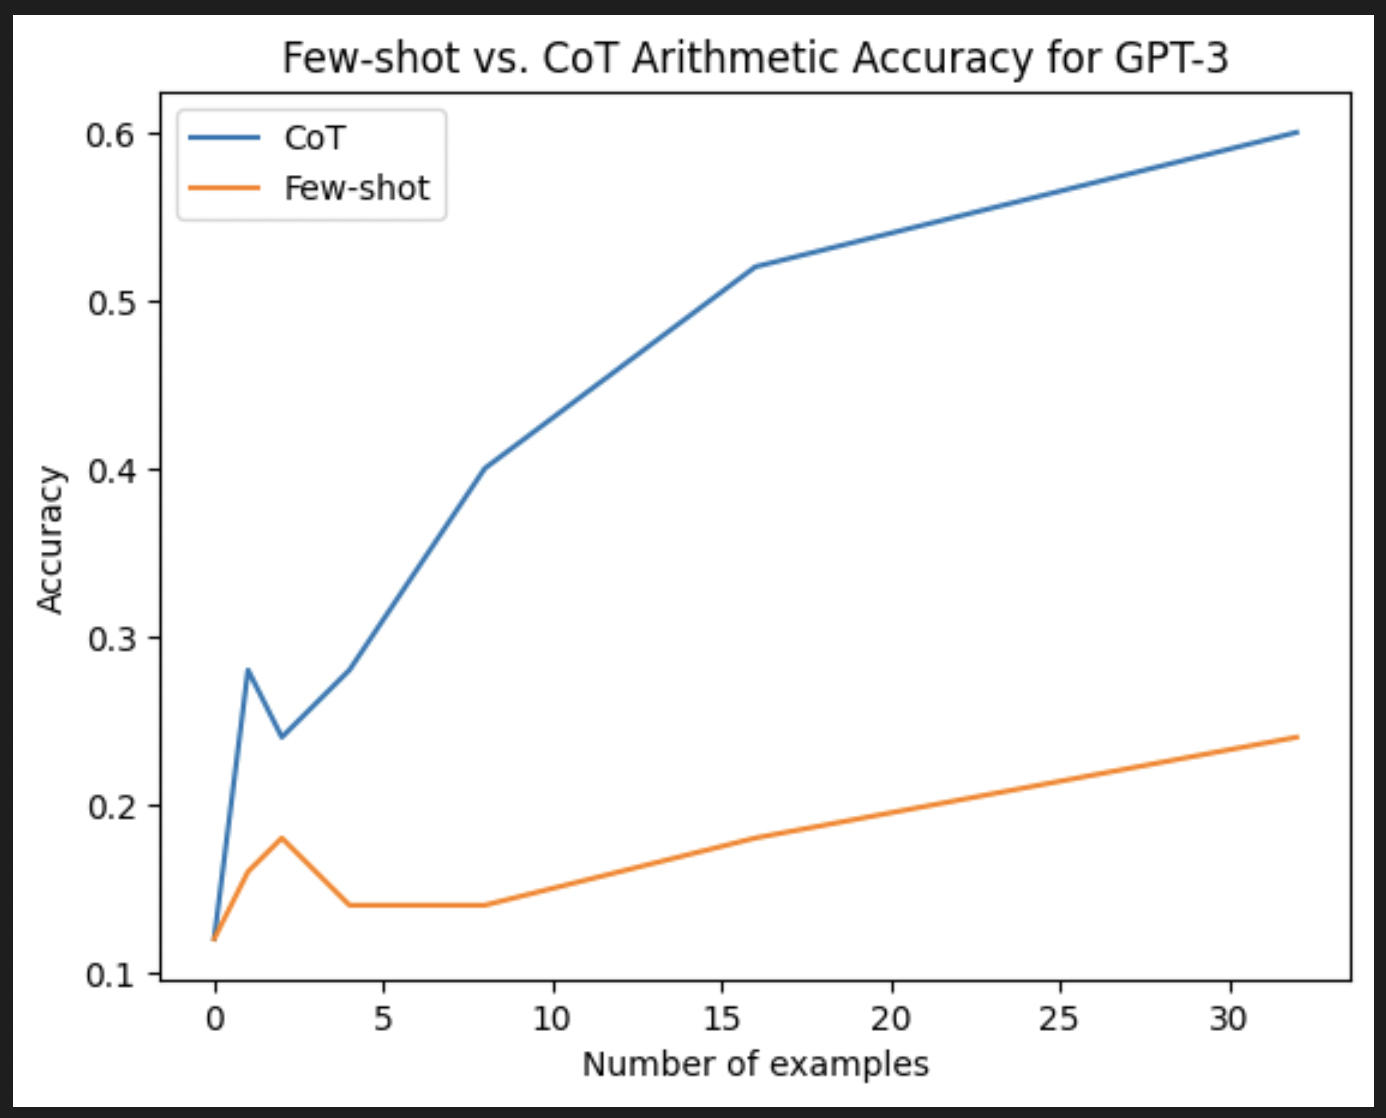
\includegraphics[width=0.75\textwidth]{chart}\\\\
As an expansion, we also included 0 examples in order to benchmark the baseline performance of our instruction-tuned LLMs to zero-shot calculate the value of the arithmetic expression.

What we can see is that increasing the number of examples improves the language model's ability to arithmetic, and the chain-of-thought prompts do increasingly better than the regular few-shot prompts as the number of examples increases. I assume this is because the chain-of-thought prompts are able to better guide the language model to the correct sequence of operations required to calculate the answer, and the more examples there are, the more the language model is able to learn from the prompts.

Another interesting pattern from the chart is is a slight local maximum in performance at 2 examples, which is present for both our few-shot examples and our chain-of-thought examples. We're not sure why this maximum exists precisely at 2 examples, as directly afterward the performance drops and then increases again.
\end{document}
